% CAPITULO 1-------------------------------------------------------------------

\chapter{QUALIDADE - INTRODUÇÃO}
\label{sec:qualidade}

Existem muitas definições de qualidade de software propostas na literatura, sob diferentes pontos de vista. Qualidade é um termo que pode ter diferentes interpretações

Definição Peters (2002): "\textit{Qualidade de software é avaliada em termos de atributos de alto nível chamados fatores, que são medidos em relação a atributos de baixo nível chamados de critérios}".

Definição Sanders (1994): "\textit{Um produto de software apresenta qualidade dependendo do grau de satisfação das necessidades dos clientes sob todos os aspectos do produto}".

Definição Pressman: "\textit{Qualidade de software é a conformidade a requisitos funcionais e de desempenho que foram explicitamente declarados, a padrões de desenvolvimento claramente documentados, e a características implícitas que são esperadas de todo software desenvolvido por profissionais}".

Definição ISO9126 (1994): "\textit{Qualidade é a totalidade de características e critérios de um produto ou serviço que exercem suas habilidades para satisfazer às necessidades declaradas ou envolvidas"}
\cite{univasf}
\nocite{usp}
\nocite{devmedia}


\section{Definições de Qualidade}
\label{sec:tradicional}

O conceito da qualidade tem hoje importância fundamental para alavancar a competitividade das empresas. Atualmente, a preocupação com a qualidade deixou de ser um diferencial competitivo e passou a ser um pré-requisito básico para participação no mercado. No setor de \textit{software} não é diferente. A disseminação do uso do \textit{software} em todas as áreas, envolvendo monitoração, controle e gestão de funções críticas, tem aumentado consideravelmente a importância da qualidade de \textit{software}.

Podemos definir qualidade sob o aspecto de três pilares, que são:

Os requisitos de software são a base na qual a qualidade é medida.
A falta de conformidade com os requisitos significa falta de qualidade.

Padrões especificados definem um conjunto de critérios de desenvolvimento que
orientam a maneira segundo a qual o software passa pelo trabalho de engenharia.
Se os critérios não forem seguidos, o resultado quase que seguramente será a falta
de qualidade.

Existe também um conjunto de requisitos implícitos que frequentemente não são mencionados na especificação. Por exemplo, o desejo de uma boa Integridade no acesso ao Sistema.

\section{Qualidade}

Qualidade hoje em dia não é apenas um diferencial de mercado para a empresa conseguir vender e lucrar mais, é um pré-requisito que a empresa deve conquistar para conseguir colocar seu produto no mercado global. Apesar da ideia de qualidade parecer aparentemente intuitiva, quando analisada com maior atenção, o conceito se revela um pouco mais complexo.

Conceituar qualidade de fato é uma tarefa complexa, mas ela pode ser vista como um método gerencial que através de procedimentos disseminados por toda a organização, busca garantir um produto final que satisfaça às expectativas do cliente, dentro daquilo que foi acordado inicialmente.

Garantia de qualidade: consiste nas funções gerenciais de auditar e relatar.

Controle de qualidade: envolve a série de inspeções, revisões e testes usados ao
longo do processo de \textit{software} para garantir que cada produto de trabalho satisfaça os requisitos estabelecidos para ele.

\begin{figure}[H]
    \centering
    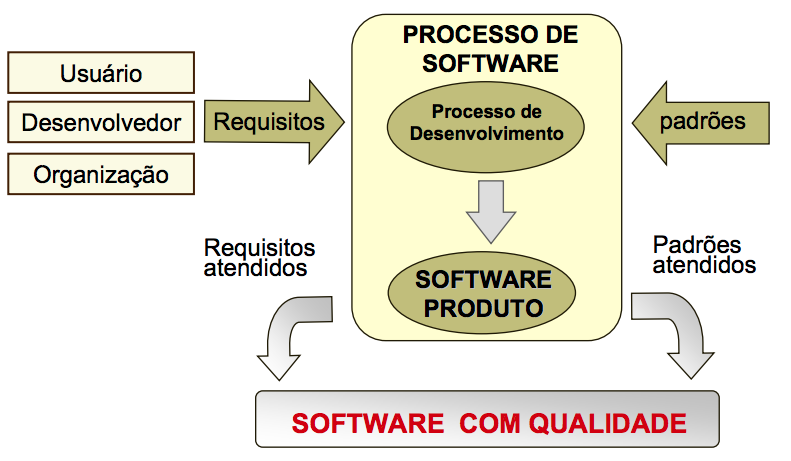
\includegraphics[width=0.7\linewidth]{dados/figuras/qualidade}
    \caption{Ciclo de qualidade}
    \label{fig:qualidade}
\end{figure}

\section{Modelo de Qualidade CMM - Capability Maturity Model }
\label{cmm}

Conhecido como "Modelo de Maturidade da Capacidade", o CMM é uma iniciativa
do SEI (Software Engineering Institute) para avaliar e melhorar a capacitação de empresas
que desenvolvem software [EDS Quality Plan, 2004]. O projeto CMM foi apoiado pelo
Departamento de Defesa do Governo dos Estados Unidos, que é um grande consumidor de
software e precisava de um modelo formal que permitisse selecionar os seus fornecedores
de software de forma adequada.

Embora não seja uma norma emitida por uma instituição internacional (como a ISO
ou o IEEE), esta norma tem tido uma grande aceitação mundial, até mesmo fora do
mercado americano. O modelo, publicado em 1992, pode ser obtido na própria Internet com
facilidade. O CMM também é chamado de SW-CMM (Software CMM).

\section{Maturidade}

O CMM é um modelo para medição da maturidade de uma organização no que diz
respeito ao processo de desenvolvimento de software. A definição do que é "Maturidade"
pode ser melhor entendida através da análise da figura abaixo.

\begin{figure}[H]
    \centering
    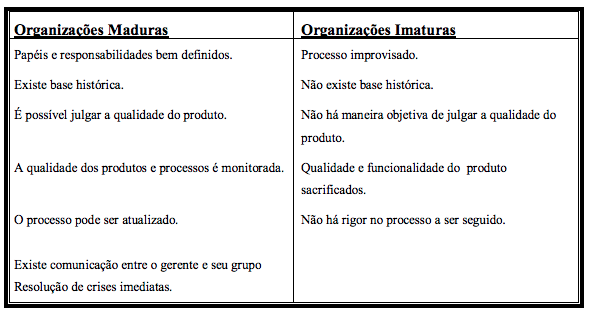
\includegraphics[width=0.7\linewidth]{dados/figuras/maturidade}
    \caption{Organizações Maduras x Organizações Imaturas}
    \label{fig:qualidade}
\end{figure}

\section{Níveis}

O CMM classifica as organizações em cinco níveis distintos, cada um com suas
características próprias. No nível 1, estão as organizações mais imaturas, onde não há
nenhuma metodologia implementada e tudo ocorre de forma desorganizada. Por outro lado,
no nível 5 estão as organizações mais maduras, onde cada detalhe do processo de
desenvolvimento está definido, quantificado e acompanhado e a organização consegue até
absorver mudanças no processo sem prejudicar o seu desenvolvimento.

\subsection{Nível 1 – Inicial}

O processo de desenvolvimento é desorganizado e caótico. Poucos
processos são definidos e o sucesso depende de esforços individuais e heróicos. O processo
de software de uma organização de Nível 1 é imprevisível porque é constantemente
alterado ou modificado à medida que o trabalho progride. Os cronogramas, os orçamentos,
as funcionalidades e a qualidade do produto são geralmente imprevisíveis. O desempenho
depende da capacidade dos indivíduos e varia com as suas habilidades, conhecimentos e
motivações inatas. Existem poucos processos de software estáveis em evidência e o
desempenho só pode ser previsto através da habilidade individual ao invés da capacidade
da organização;

\subsection{Nível 2 - Repetível}

Os processos básicos de gerenciamento de projeto estão estabelecidos e permitem acompanhar custo, cronograma e funcionalidade. Os projetos nas organizações de nível 2 têm instalado controles básicos de gestão de software. Os compromissos do projeto são baseados em resultados observados em projetos anteriores e nos requisitos do projeto atual. Os gerentes do projeto acompanham os custos, os cronogramas e as funcionalidades do software. Os problemas com compromissos são identificados quando surgem. Os requisitos de software e os produtos de trabalho desenvolvidos para satisfazê-los são congelados e a integridade dos mesmos é controlada. Os padrões do projeto de software são definidos e a organização garante que eles sejam seguidos fielmente. O projeto de software trabalha com os seus subcontratados, se existirem, para estabelecer uma forte relação cliente-fornecedor.

\subsection{Nível 3 - Definido}

Tanto as atividades de gerenciamento quanto de engenharia do
processo de desenvolvimento de software estão documentadas, padronizadas e integradas
em um padrão de desenvolvimento da organização. Todos os projetos utilizam uma versão
aprovada e adaptada do processo padrão de desenvolvimento de software da organização.
A capacidade do processo de software das organizações de nível 3 pode ser resumida como
sendo padrão e consistente porque a engenharia de software e as atividades de gestão são
estáveis e repetíveis. Dentro de linhas estabelecidas de produtos, o custo, o cronograma e as funcionalidades estão sob controle e a qualidade de software é acompanhada.

\subsection{Nível 4 - Gerenciado}

São coletadas medidas detalhadas da qualidade do produto e
processo de desenvolvimento de software. Tanto o produto quanto o processo de
desenvolvimento de software são entendidos e controlados quantitativamente. A capacidade
do processo de software das organizações de nível 4 pode ser resumida como sendo
previsível porque o processo é medido e opera dentro de limites mensuráveis. O processo
desse nível permite que a organização antecipe as tendências na qualidade dos produtos e
dos processos dentro das fronteiras quantitativas desses limites. Quando esses limites são
excedidos, são tomadas ações para corrigir a situação. Os produtos de software são, como
era de se esperar, de alta qualidade;

\subsection{Nível 5 - Otimizado}

O nível de maturidade 5 se concentra no melhoramento contínuo do
desempenho de processos através de melhorias tecnológicas incrementais e inovadoras. Os
objetivos quantitativos de melhoria de processos para a organização são estabelecidos,
continuamente revisados para refletir alterações nos objetivos do negócio. O melhoramento
contínuo é conseguido através de um \textit{feedback} dos processos e pelo uso pioneiro de
tecnologias inovadoras.

\begin{figure}[H]
    \centering
    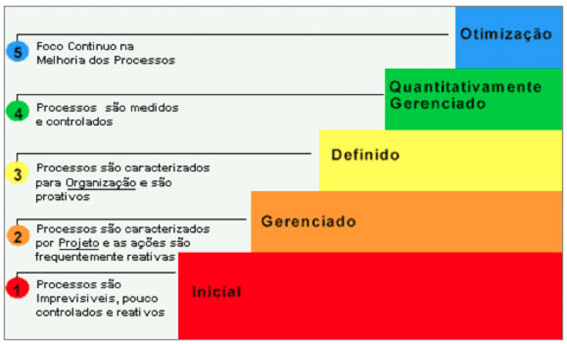
\includegraphics[width=0.7\linewidth]{dados/figuras/cmm}
    \caption{Níveis de Maturidade [SEI, Software Engineering Institute]}
    \label{fig:cmm}
\end{figure}

\nocite{cmmcmmi}

\section{Entendendo os níveis de maturidade}

O modelo CMM descreve atributos essenciais (ou chaves) que seriam esperados
para caracterizar uma organização em um nível de maturidade [Maldonado,2001]. É um
modelo normativo, no sentido de que as práticas detalhadas caracterizam os tipos normais
de comportamento que seriam esperados em uma organização que desenvolve projetos em
larga escala em um contexto de contratação governamental. A intenção é que o CMM tenha
um nível suficiente de abstração que não restrinja desnecessariamente a maneira que o
processo de software é implementado pela organização: ele simplesmente descreve o que
normalmente seria esperado que os atributos essenciais do processo de software fossem.

\section{CMMI}

A experiência no uso do CMM durante uma década serviu para identificar pontos
em que o modelo poderia ser melhorado. Ao mesmo tempo, o surgimento do projeto SPICE
(Software Process Improvement and Capability Determination), da ISO, levou à
necessidade de compatibilização do CMM com a futura norma ISO 15504, que será o
resultado do projeto. Por estas razões, o SEI iniciou um projeto chamado CMMI (CMM
Integration).

O CMMI é um modelo para definir e melhorar a capacidade e a maturidade dos
processos das organizações que produzem software. As empresas que investem no CMMI
têm como principais benefícios o aumento da qualidade dos processos de software e o
reconhecimento internacional dessa qualidade. Também têm uma maior e mais efetiva gerência de projetos de software, no que diz respeito a custo, tempo e recursos utilizados.
Esse modelo possibilita uma redução significativa de defeitos nos serviços gerados e
maior qualificação do pessoal no atendimento ao cliente, além da customização dos
processos de acordo com as necessidades. Com isso, as empresas reduzem o retrabalho,
baixam seus custos e agilizam suas soluções, agregando valor para o cliente.

Os objetivos do CMMI são, basicamente, voltados para a redução do custo da
implementação de melhoria de processo. São eles [Ahern, 2001]:

\begin{itemize}
    \item Eliminação de inconsistências e redução de duplicidades;
    \item  Melhoria da clareza e entendimento;
    \item  Utilização de terminologia comum e estilo consistente;
    \item  Estabelecimento de regras de construção uniformes;
    \item  Manutenção de componentes comuns;
    \item  Consistência com a futura norma ISO/IEC 15504;
    \item  Sensibilidade às implicações dos esforços legados.
\end{itemize}

A busca pela certificação CMMI representa a afirmação da filosofia de
aprimoramento contínuo dos produtos e a concretização de um importante passo rumo à
exportação de software.

A principal mudança do CMMI em relação ao CMM é a possibilidade de utilização
de duas diferentes abordagens para a melhoria de processos. Estas duas abordagens são
conhecidas como o “representação contínua” e o “representação em estágios”. Existem
muitas razões para uma empresa selecionar uma representação ou outra. Pode ser que uma
organização escolha utilizar a representação que lhe seja mais familiar.

O projeto CMMI envolveu uma grande quantidade de pessoas de diferentes
organizações do mundo todo. Estas organizações utilizavam um modelo CMM ou
múltiplos CMMs e estavam interessadas nos benefícios do desenvolvimento de um
framework integrado para auxiliar a melhoria de processos no âmbito do
empreendimento como um todo.

O trabalho do projeto CMMI é patrocinado pelo Departamento de Defesa dos
Estados Unidos (Department of Defense – DoD), especificamente pelo departamento da
Sub-Secretaria de Defesa, Aquisição, Tecnologia e Logística (Office of the Under
Secretary of Defense, Acquisition, Technology, and Logistics - OUSD/AT\&L). O
patrocínio da indústria é garantido pelo Comitê de Engenharia de Sistemas da
Associação Industrial da Defesa Nacional (National Defense Industrial Association -
NDIA).

O produto de software passa a ser , cada vez mais, um componente comum em uma
série de outros produtos, desde carros, eletrodomésticos, elevadores, telefones, até sistemas de informação organizacionais. De um produto exige-se qualidade e preço. Portanto, como produto, o software deve ter o nível de qualidade exigido e procurar ser desenvolvido com o menor custo possível.

Produzir software de qualidade é uma meta básica da engenharia de software, que
disponibiliza métodos, técnicas e ferramentas para esse fim. Muito tem sido escrito sobre
qualidade e seus vários adjetivos. No entanto, o fundamental é que o software seja
confiável, ou seja, que seja eficaz e siga os padrões exigidos pelo contexto onde irá atuar.
Cada vez mais a sociedade pressiona o setor de software para que a característica
“qualidade” seja preponderante. Normas internacionais como a ISO e iniciativas como as
do SEI (Software Engineering Institute) são exemplos disso.

Devemos sempre ter em mente que a produção de software é um processo que envolve,
como parte fundamental, seres humanos. As tecnologias de produção de software, tem por
objetivo automatizar ao máximo a produção, mas ainda são fundamentalmente dependentes
da qualidade das equipes, das pessoas, de todo o time envolvido num processo de
desenvolvimento.

\nocite{cmmcmmi}
